\section{CPN Tools}
CPN Tools \cite{RefWorks:87} is a tool for editing, simulating, and doing state space and performance analysis of CPN models. The ProPCPN models presented in this thesis are constructed using CPN Tools. In Fig.~\ref{fig:cpntools} we show a screenshot of the producer-consumer model in CPN Tools. The user works directly with the graphical representation of the model, e.g., a transition can be drawn using the rectangle in the tool box shown in the upper right corner of Fig.~\ref{fig:cpntools}. The model is being checked for errors continuously to assist the user in the construction of CPN models. ProPCPNs, being a subclass of CPNs, can be created and analysed in CPN Tools just like any other CPN model. 

\ignore{In the current version it is the modellers responsibility that the model is in fact a ProPCPN model.}   

\begin{figure}[b!]
\centering
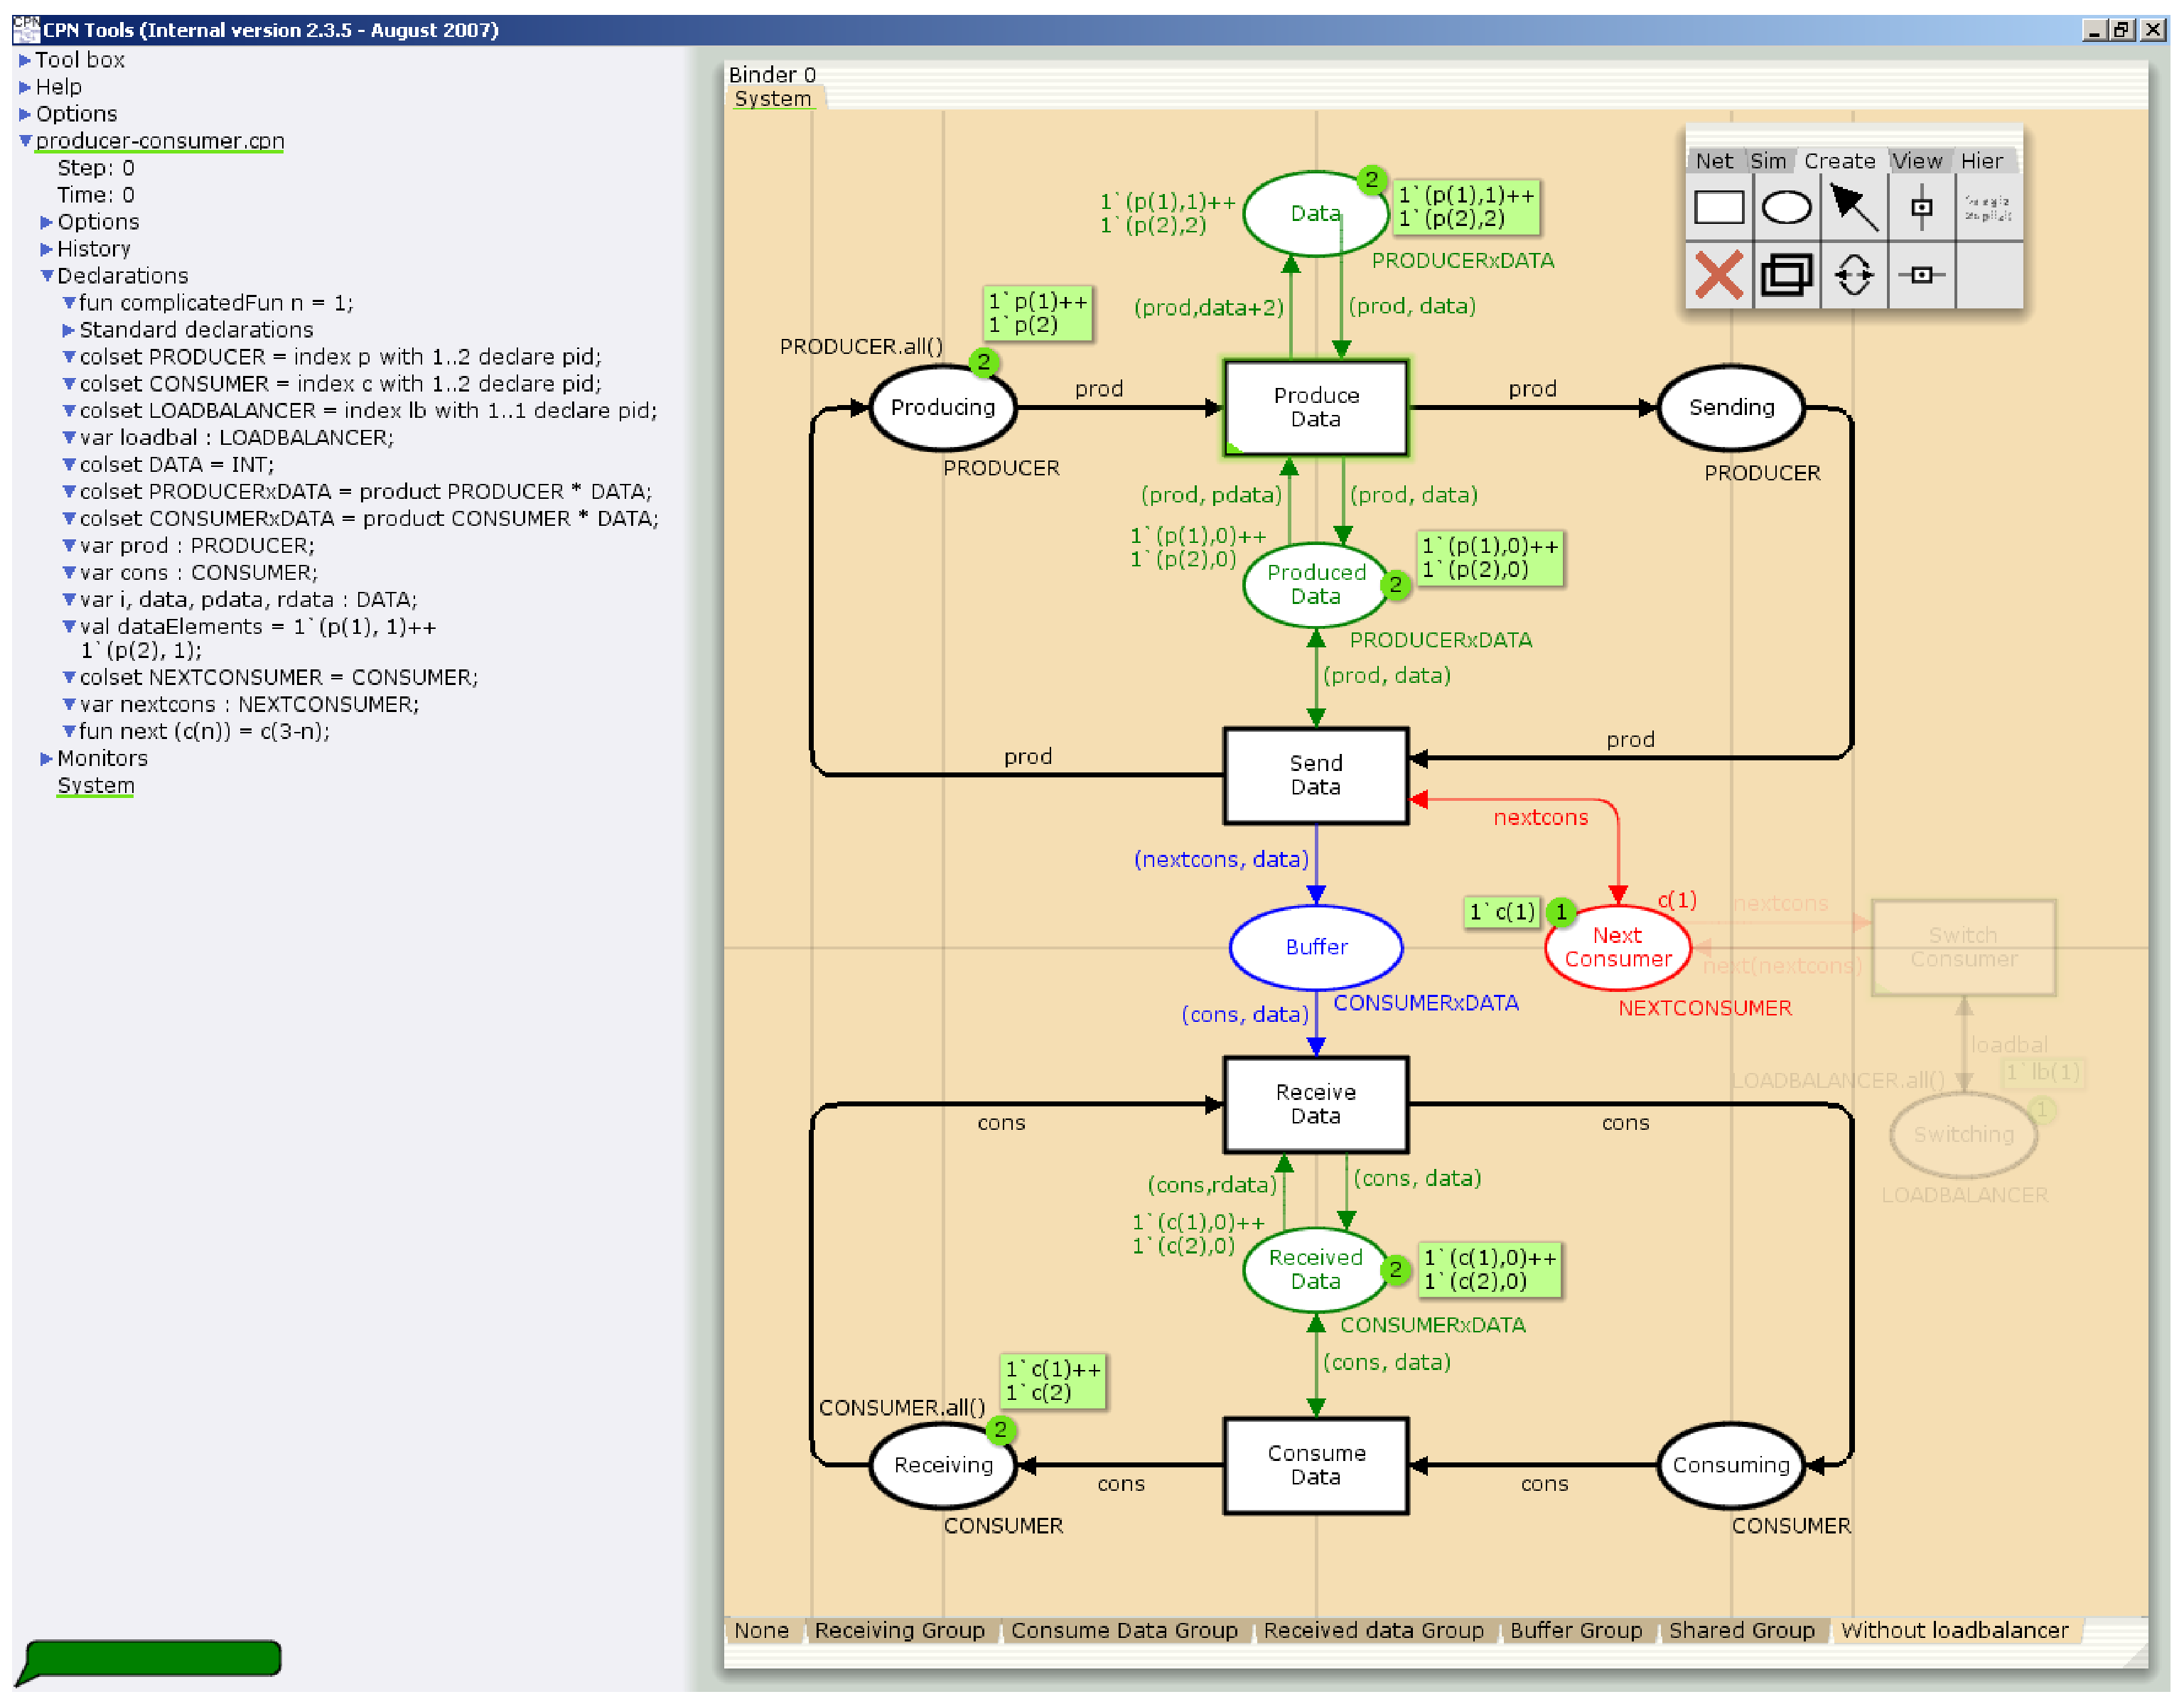
\includegraphics[width=\textwidth]{techniques_and_tool/graphics/CPNTools.eps}
\caption{The producer-consumer model in CPN Tools}
\label{fig:cpntools}
\end{figure}
